\documentclass[00_complete]{subfiles}

%\documentclass[12pt]{report}
\usepackage[utf8]{inputenc}
\usepackage{amsmath,amssymb,amsthm,gensymb,parskip,graphicx,footmisc,csquotes,enumerate,datetime2}
\usepackage[]{libertinus}
\usepackage[breaklinks]{hyperref}
\hypersetup{
  pdfauthor={Moshe Krumbein},
  colorlinks=true,
  linkcolor={black},
  filecolor={black},
  citecolor={black}, %blue
  urlcolor={black}, %blue
}
\usepackage[top=30mm,bottom=30mm,left=30mm,right=30mm]{geometry}
%\setlength{\emergencystretch}{2em} % prevent overfull lines
\providecommand{\tightlist}{%
\setlength{\itemsep}{0pt}\setlength{\parskip}{0pt}}

\renewcommand\qedsymbol{$\blacksquare$}

\theoremstyle{definition}
\newtheorem*{definition}{Definition}
\newtheorem*{theorem}{Theorem}
\newtheorem*{axiom}{Axiom}
\newtheorem*{lemma}{Lemma}

\theoremstyle{remark}
\newtheorem*{note}{Note}
\newtheorem*{symbols}{Symbol}
\newtheorem{example}{Example}[section]
\newtheorem*{claim}{Claim}
\newtheorem*{conclusion}{Conclusion}
\newtheorem*{reminder}{Reminder}

\usepackage{fancyhdr}
\usepackage[italicdiff]{physics}
\MakeOuterQuote{"}

\renewcommand{\chaptermark}[1]{\markboth{#1}{}}

\pagestyle{fancy}

\setlength{\headheight}{14.5pt}
\addtolength{\topmargin}{-2.5pt}

\fancyhf{}
\rhead{Moshe Krumbein}
\lhead{\chaptermark}
\cfoot{\thepage}
\fancyhead[R]{\chaptername~\thechapter}
\fancyhead[L]{\mbox{\leftmark}}

\usepackage[Rejne]{fncychap}
\usepackage{titling}

\makeatletter
\renewcommand{\@chapapp}{\vspace*{-100pt}\huge\thetitle}
\makeatother

\makeatletter
\newcommand{\subtitle}[1]{%
  {\center\vspace*{-60pt}%
  \linespread{1.1}\Large\scshape#1%
  \par\nobreak\vspace*{35pt}}
}
\makeatother

\newcommand{\Chapter}[2]{
    \def\n{#2}
    \setcounter{chapter}{\the\numexpr\n-1}
    \chapter{#1}
    \subtitle{\theauthor~- \thedate}
}

\DeclareMathOperator{\Ima}{Im}
\DeclareMathOperator{\Id}{Id}
\DeclareMathOperator{\cis}{cis}

\newcommand{\Mod}[1]{\ (\mathrm{mod}\ #1)}
\newcommand{\st}[0]{\;\mathrm{s.t.}\;}


\title{Mathematical Methods}
\author{Moshe Krumbein}
\date{Fall 2021}

\begin{document}
\Chapter{Integration of Multivariable Functions}{12}

\section{Double Integrals}
Given the function $z=f(x,y)$ and the domain $D$ on the plane. We want to find:
$$\iint\limits_Df(x,y)=\iint f(x,y)\dd{y}\dd{x}$$
Which is essentially the volume of the domain between $D$ and $f$.
\begin{definition}[Fubini's theorem]
    If $D=[a,b]\times[c,d]$:
    $$\iint\limits_D f \dd{A}= \int_{a}^{b}\int_{c}^{d}
    f(x,y)\dd{y}\dd{x}=\int_{c}^{d}\int_{a}^{b} f(x,y)\dd{x}\dd{y}$$
\end{definition}
\begin{example}
    \begin{gather*}
        f(x,y)=x^2+3y^2+xy \quad D=[1,2]\times[0,1] \\
        \iint\limits_D f\dd{A} =
        \int_{0}^{1}\left(\int_{1}^{2}(x^2+3y^2+xy)\dd{x}\right)\dd{y} =
        \int_{0}^{1}\left(\frac{x^3}{3}+3xy^2+\frac{x^2}{2}y\right)\Biggr|_{x=1}^2\dd{y}
        \\
        \int_{0}^{1}\left(\frac{7}{3}+3y^2+\frac{3}{2}y\right)\dd{y}
        =\frac{49}{12}
    \end{gather*}
\end{example}
\begin{note}
    If $f(x,y)=g(x)h(y)$ and $D=[a,b]\times[c,d]$:
    $$\iint\limits_Df(x,y)=\int_{a}^{b}\left(\int_{c}^{d}g(x)h(y)\dd{y}\right)\dd{x}
    \int_{a}^{b}g(x)\int_{c}^{b}h(y)\dd{y}\dd{x} =
    \int_{a}^{b}g(x)\dd{x}\cdot\int_{c}^{d}h(y)\dd{y}
    $$
\end{note}
\section{Double Integrals of Non-rectangular Domains}
\emph{Simple Vertical Domain}:
\begin{gather*}
    a \leq x \leq b \quad g(x) \leq y \leq h(x) \\
    \iint\limits_D f= \int_{a}^{b}\int_{g(x)}^{h(x)}f(x,y)\dd{y}\dd{x}
\end{gather*}
\emph{Simple Vertical Domain}:
\begin{gather*}
    c \leq y \leq d \quad g(y) \leq x \leq h(y) \\
    \iint\limits_D f= \int_{c}^{d}\int_{g(y)}^{h(y)}f(x,y)\dd{x}\dd{y}
\end{gather*}
\section{Uses of Double Integrals}

\subsection{Volume of Solids of Revolution}

In essence, to find the area of a solid of revolution, we consider the volume
to be the sum of thin disks with the radius on $f(x)$:
$$\lim \sum_{k=1}^{\infty} \underbrace{\pi(f(x))^2}_{\text{area of the
circle}}\Delta x_k=\pi\int_{a}^{b}(f(x))^2\dd{x}$$
    \begin{figure}[ht]
    \centering
    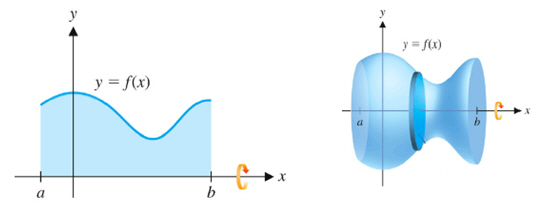
\includegraphics[width=0.66\textwidth]{w12_solid}
    \caption{Volume of Solids of Revolution}
    \end{figure}
\subsection{Center of Gravity}

\begin{gather*}
    \text{Mass: } \iint\limits_D f(x,y)\dd{x}\dd{y} \\
    \text{Center of Mass:} \\
    \overline x = \frac{\iint x\cdot f(x,y)\dd{x}\dd{y}}{\text{mass}} \\
    \overline y = \frac{\iint y\cdot f(x,y)\dd{x}\dd{y}}{\text{mass}}
\end{gather*}
\subsection{Useful Formulas}
\begin{gather*}
    \int_{a}^{b}1\dd{x}=\underbrace{b-a}_{\text{length}} \\
    \iint\limits_D 1\dd{x}\dd{y}=\text{ Area of $D$} \\
\end{gather*}
\begin{example}
    $$\int_{-6}^{6}\int_{0}^{\sqrt{26-x^2}}1\dd{x}\dd{y}$$
    This may be solved in the conventional way, though it'll take some time.
    However we can just consider the area of the domain which is the upper
    half of a circle with a radius of $3$, giving us:
    $$\frac{1}{2}\pi 6^2 = 18\pi$$
\end{example}
\section{Triple Integrals}
$$D \subseteq \mathbb{R}^3 \quad \iiint\limits_Df(x,y,z)\dd{v}$$
What does it represent?

If $f(x,y,z)$ is the density, then the integral is the mass.

If $f(x,y,z)\equiv 1$, then the integral is the volume of the domain.
\begin{example}
    \begin{gather*}
        f(x,y,z)=x+yz \quad D=[1,3]\times [0,1]\times[-2,6] \\
        \int_{1}^{3}\int_{-2}^{6}\int_{0}^{1} (x+yz)\dd{y}\dd{z}\dd{x} =
        \int_{1}^{3}\int_{-2}^{6}\underbrace{[xy+\frac{y^2a}{2}]\Bigr|_{y=0}^{1}}_{x+\frac{z}{2}}\dd{z}\dd{x}
        \\ \vdots
    \end{gather*}
\end{example}
\begin{example}
    \begin{gather*}
        \iiint\limits_D xyz \dd{v} \quad D: x=0,y=0,z=0, x+2y+z=1 \\
        0 \leq z \leq 2-x-2y \quad 0 \leq y \leq \frac{1}{2}-\frac{1}{2}x \quad
        0 \leq x \leq 1 \\
        \int_{0}^{1}\int_{0}^{\frac{1}{2}-\frac{1}{2}x}\int_{0}^{2-x-2y}xyz\dd{z}\dd{y}\dd{x}
        \\ \vdots
    \end{gather*}
\end{example}
\section{Change of Coordinates in Integrals}
Similar to finding the area of a function after changing coordinates using the
\emph{Jacobean}, when we change coordinates on a double (or triple) integral:
$$\dd{x}\dd{y}=|J|\dd{u}\dd{v}$$
\begin{example}
    \begin{gather*}
        f(x,y)=x+1 \quad D: y<x, x<\sqrt{1-y^2} \\
        \iint\limits_D(x+1)\dd{x}\dd{y}
    \end{gather*}
    Let's convert this to the polar coordinate system:
    \begin{gather*}
        0 \leq r \leq 1 \quad 0 \leq \theta \leq \frac{\pi}{4} \\
        \int_{0}^{1}\int_{0}^{\frac{\pi}{4}}(1+r\cos\theta)r\dd{r}\dd{\theta}
    \end{gather*}
\end{example}

\end{document}
